\documentclass[10pt,conference,compsocconf]{IEEEtran}


\usepackage{amsmath}    % math
\usepackage{graphicx}   % For figure environment
\usepackage{todonotes}
\usepackage{subcaption}

\usepackage{hyperref}
\begin{document}
\title{Mini-project II}

\author{
  Ada Pozo P\'{e}rez, Luc\'{i}a Montero Sanchis, Milica Novakovic\\
  \textit{Deep Learning 2018, EPFL Lausanne, Switzerland}
}

\maketitle

\begin{abstract}
  This report describes the implementation of a simple deep learning framework. Several different optimizers, activation functions, layers and loss functions are implemented, including fully connected, dropout, \textit{ReLU}, \textit{Tanh}, sequential and \textit{MSE} loss among others. This framework is used for testing different architectures on a toy dataset, using different optimizers, in order to determine the effects that different activation functions and optimizers have in the training and accuracy.
\end{abstract}

\section{Introduction}
	In this project we implement a deep learning framework using only \textit{Pytorch} tensors and \textit{numpy}.
	
	The framework is built with two base classes: \textit{Module} and \textit{Optimizer}. The following containers are implemented as subclasses for them:
	
	\begin{itemize}
	    \item Layers: \textit{Linear}, \textit{Sequential} and \textit{Dropout}.
	    \item Activation functions: \textit{ReLU}, \textit{Leaky ReLU}, \textit{Sigmoid} and \textit{Tanh}.
	    \item Loss functions: \textit{Mean Squared Error (MSE)} and \textit{Cross-entropy loss}.
	    \item Optimizers: \textit{Stochastic Gradient Descent} and \textit{Adam}.
	\end{itemize}
	
    To test our framework we generate a toy dataset and run several experiments on it, comparing the performance of different combinations of modules, activations, optimizers and loss functions.
    
    The rest of this report is organized as follows: Section \ref{sec:implementation} describes how the different containers were implemented while Section \ref{sec:experiments} shows the results of the experiment to test the framework. Conclusions are drawn in Section \ref{sec:summary}. 
	
\section{Implementation} % (fold)
\label{sec:implementation}
    We have defined two generic classes, \textit{Module} and \textit{Optimizer}, that are used as parent classes for the implementations. The optimizers are based on the structure of \textit{Optimizer}, whereas the remaining implementations are based on \textit{Module}.
    
    \textit{Optimizer} has two methods: 
    \begin{itemize}
        \item \textit{step}: implements the update of the parameters.
        \item \textit{adaptive\_lr}: returns a generator that decays the learning rate by a factor with every optimization step.
    \end{itemize}
    
    In \textit{Module} we can find the methods:
    \begin{itemize}
        \item \textit{forward} and  \textit{backward}: implement the forward and backward passes of backpropagation, respectively.
        \item \textit{update}: updates the values of the parameters and resets the computed gradients to zero.
        \item \textit{params}: returns the values and the last computed gradients of the parameters of the layer.
    \end{itemize}

  \subsection{Layers} % (fold)
  \label{sub:modules}
    % Not sure about having ``modules'' as a title here
    \subsubsection{Linear} % (fold)
    \label{ssub:linear}
        The fully connected layer is implemented in the \textit{Linear} module. It is created specifying the number of input and output units. It is also possible to specify the default learning rate, which will be used to update the parameters. Nevertheless, this learning rate is only used when no learning rate is specified for the \textit{update} function.
        
        Unless a specific standard deviation (std) is specified during initialization, the weights are initialized with the Xavier \cite{Glorot10understandingthe} initialization adapted for ReLU \cite{DBLP:journals/corr/HeZR015} -- following a zero-mean Gaussian distribution with standard deviation given by $\text{std} = \sqrt{2/n}$,
        where $n$ is the number of input units.
        If a value for parameter \textit{std\_w} is specified, then the weights are initialized according to the zero-mean Gaussian distribution whose std value is \textit{std\_w}. For instance, when using $\tanh$ or sigmoid activation functions we recommend to specify a value for the parameter equal to $\text{std} = 1\sqrt{n}$.
  	
        In addition to this, in the initialization it is also specified whether there is a bias -- in which case the bias values would be initialized following a Gaussian distribution with zero mean and standard deviation given by the parameter \textit{std\_b}. If the value of parameter \textit{std\_b} is not specified, they are initialized to 0. If there is no bias, in the backpropagation this parameter is ignored.
  	
        During the forward pass, the input to the layer is saved for the subsequent gradient computation. The output of the layer $s^{(l)}$ is computed with the equation \ref{eq:forward}, where $w^{(l)}$ and $b^{(l)}$ are the values of the weights and the bias respectively and $x^{(l-1)}$ is the input to the layer. The bias term is considered if it was specified to do so, otherwise it is ignored.
        \begin{equation}
      	    \label{eq:forward}
            s^{(l)} = w^{(l)}x^{(l-1)} + b^{(l)} 
        \end{equation}
     
        The backward pass function receives as an argument the gradient of the loss with respect to the output of the layer ($\partial l/\partial s^{(l)}$) and returns the gradient of the loss with respect to the input of the layer, which is computed as given by equation \ref{eq:backward_x}. The gradient of the loss with respect to the weights and with respect to the bias are computed with equations \ref{eq:backward_w} and \ref{eq:backward_s}, respectively:
         \begin{equation}
      	    \label{eq:backward_x}
            \frac{\partial l}{\partial x^{(l-1)}} =\frac{\partial l}{\partial s^{(l)}}  w^{(l)}
         \end{equation}
         \begin{equation}
      	    \label{eq:backward_w}
            \frac{\partial l}{\partial w^{(l)}} =\left(\frac{\partial l}{\partial s^{(l)}}\right)^T x^{(l-1)}
         \end{equation}
         \begin{equation}
      	    \label{eq:backward_s}
            \frac{\partial l}{\partial b^{(l)}} =\frac{\partial l}{\partial s^{(l)}}
         \end{equation}
     
        The update of the parameters is performed when the method \textit{update} is called. If a learning rate is passed as a parameter it is used for the update, otherwise the one specified upon initialization is used. As will be explained in more detail in the optimizers section \ref{sub:optimizers}, the update can be done directly on the derivatives of the bias and weights (for instance, when using SGD), or in the case when the parameter \textit{values} is specified it will use these values instead (if Adam is used, the optimizer computes the parameter \textit{values} that should be used). The equations used for the updates are therefore given by \ref{eq:update_w} and \ref{eq:update_b}, where $\gamma$ is the learning rate:
        \begin{equation} 
            \label{eq:update_w}
            w^{(l)}\leftarrow
            \begin{cases}
              w^{(l)} -  \gamma \cdot \partial l/\partial w^{(l)}, & \text{if SGD is used} \\
              w^{(l)} -  \gamma \cdot \text{value}_w, & \text{if Adam is used}
            \end{cases}
        \end{equation}
        
        \begin{equation}
            \label{eq:update_b}
            b^{(l)}\leftarrow
            \begin{cases}
              b^{(l)} -  \gamma \cdot \partial l/\partial w^{(l)}, & \text{if SGD is used} \\
              b^{(l)} -  \gamma \cdot \text{value}_b, & \text{if Adam is used}
            \end{cases}
        \end{equation}
        
        When using \textit{Adam}, $\text{value}_w$ and $\text{value}_b$ are computed as given by equation \ref{eq:valueadam}.
        
        Lastly, the \textit{Linear} module's method \textit{params} returns a list of tuples containing a tuple with the weights and the gradient and, if bias is activated, a second tuple with the values of the bias and the gradient.
    % subsubsection linear (end)

  	\subsubsection{Sequential} % (fold)
  	\label{ssub:sequential}
        This class implements a container for a list of layers. Its parameters are the list of layers and a variable that indicates whether the model is in training or testing mode. In the forward pass, it simply calls the \textit{forward} method of each layer, propagating the output through the layers. In the backward pass, it propagates the gradient calling the corresponding method of each layer iterating through them in reverse order.
        
        Likewise, the \textit{params} method calls the \textit{params} method of each layer and combines their outputs, returning a list of tuples containing the values and gradient for each parameter.
        
        The \textit{update} method iterates over all the layers calling each layer's corresponding method. If a learning rate $\gamma$ is specified, then it is used to update all parameters. It is also possible to specify the \textit{values} parameter that should be used for the update, instead of using the gradient computed during the forward pass. As previously mentioned, this is useful for implementing the Adam optimizer and will be explained later.
   	% subsubsection sequential (end)

  	\subsubsection{Dropout} % (fold)
  	\label{ssub:dropout}
        We implement a dropout layer by defining a class \textit{Dropout}. This layer is created taking as parameters the probability of dropping a hidden unit ($p_{drop}$) and whether the model is training. If it is not training, the forward and backward passes simply return their respective inputs.
        
        The forward pass is implemented in the \textit{forward} method. It creates a mask of hidden units to drop and saves it for the backward pass. The mask is used to shut down the corresponding units of the input data. Lastly, the result is normalized by $1-p_{drop}$. The \textit{backward} method carries out the backward pass, using the mask saved in the forward pass to shut down the same units of the gradient of the next layer. The result is again normalized by $1-p_{drop}$.
  	% subsubsection dropout (end)
  % subsection modules (end)

  \subsection{Activation functions} % (fold)
  \label{sub:activation_functions}
    The following activation functions are implemented in our framework:
  	\subsubsection{ReLU} % (fold)
  	\label{ssub:relu}
        In the forward pass this activation layer applies the non-linear function $f(x) = max(0,x)$ to the input \cite{Nair:2010:RLU:3104322.3104425}. The backward pass is computed with the derivative:
      	\begin{equation*} 
            f'(x)=
            \begin{cases}
              1, & \text{if}\ x>0 \\
              0, & \text{otherwise}
            \end{cases}
        \end{equation*}
  	% subsubsection relu (end)

  	\subsubsection{Leaky ReLU} % (fold)
  	\label{ssub:leakyrelu}
        We implement a parametric Leaky ReLU, which takes takes a parameter $\alpha$ and computes the forward pass as:
      	\begin{equation} 
            f(x)=
            \begin{cases}
              x, & \text{if}\ x>0 \\
              \alpha\cdot x, & \text{otherwise}
            \end{cases}
        \end{equation}
    
        In the backward pass, the gradient is given by:
      	\begin{equation} 
            f'(x)=
            \begin{cases}
              1, & \text{if}\ x>0 \\
               \alpha, & \text{otherwise}
            \end{cases}
        \end{equation}
  	
  	% subsubsection leakyrelu (end)
  	\subsubsection{Tanh} % (fold)
  	\label{ssub:tanh}
        We implement the hyperbolic tangent activation function in the class \textit{Tanh}. This class computes in the \textit{forward} method the $\tanh$ of the input, which is saved for the next step. In the backward pass step, we compute the gradient as $1-\tanh^2{x}$
  	% subsubsection tanh (end)
  	\subsubsection{Sigmoid} % (fold)
  	\label{ssub:sigmoid}
        We implement the forward pass of this function using the $\tanh$ function to ensure that there is no overflow, according to the formula $\sigma(x) = 0.5 + 0.5\cdot\tanh{(x/2)}$. We store the obtained value and then compute the derivative as $\sigma(x) \cdot (1-\sigma(x))$. 
  	% subsubsection sigmoid (end)
  % subsection activation_functions (end)
  \subsection{Loss functions} % (fold)
  \label{sub:loss_functions}
  
  Two loss functions are implemented in this framework: the Mean Squared Error (MSE) and the Cross Entropy Loss.
  	\subsubsection{Mean Squared Error (MSE)} % (fold)
  	\label{ssub:mean_squared_error}
        In the forward pass, this module computes the difference between the output of the network $f(x,w)$ and the ground truth $y$ and saves it for the backward pass. The loss returned is computed as:
      	\begin{equation} 
      	Loss = \sum_{i=1}^{N}(y_i - f(x_i,w))^2
      	\end{equation} 
      	
      	The backward pass returns the gradient of the loss, which is computed using the stored difference between the output of the network and the ground truth:
      	\begin{equation} 
      	    \nabla_{Loss} = 2 (y - f(x,w))
      	\end{equation} 
  	% subsubsection mean_squared_error (end)
  	\subsubsection{Cross-entropy loss} % (fold)
  	\label{ssub:cross_entropy_loss}
  	This module computes the loss of the network in the forward pass as: 
  	\begin{equation}  
  	    Loss = -\sum_{i=1}^{N} y_i\log (f(x_i,w)) + (1 - y_i)\log(1 - f(x_i,w))
  	\end{equation} 
  	
  	In the backward pass the gradient of the loss is computed with the following equation:
  	\begin{equation}  
  	    \nabla_{Loss} =  y - f(x,w)
  	\end{equation} 
  	% subsubsection cross_entropy_loss (end)
  % subsection loss_functions (end)
  \subsection{Optimizers} % (fold)
  \label{sub:optimizers}
  As explained in the beginning of Section \ref{sec:implementation}, the optimizers are defined using a class with a \textit{step} method that updates the parameters and a method \textit{adaptive\_lr} that implements a generator that yields decaying learning rates. The decay is controlled by parameters $\kappa$ and $\eta$ according to: 
    \begin{equation}
    \label{eq:lr}
  	    \gamma^{(t)} =  \eta\cdot t^ {-\kappa}
  	\end{equation} 
  	where $t$ is incremented every time the generator is called.
  	\subsubsection{Stochastic Gradient Descent (SGD)} % (fold)
  	\label{sub:stochastic_gradient_descent_}
        The parameter update using Stochastic Gradient Descent calls the \textit{update} method of the model (explained in Sections \ref{ssub:linear} and \ref{ssub:sequential}). This update can be done either with a fixed learning rate if $\kappa$ and $\eta$ are not passed as parameters when creating the optimizer, or with the described decaying learning rate if they are passed. In the second case, each time \textit{step} is called the next learning rate is generated and passed to the \textit{update} method of the model.
  	% subsection stochastic_gradient_descent_ (end)
  	\subsubsection{Adam} % (fold)
  	\label{ssub:adam}
        This class is implemented as described in \cite{kingma2014adam}.  Given the parameters of the optimizer settings $\beta_1$, $\beta_2$ and $\epsilon$, at each timestep $t$ we first calculate the gradient with respect to the stochastic objective $g_t$ and then the first and second moment vectors are computed according to equations \ref{eq:fmv} and \ref{eq:smv} respectively:
  		\begin{equation} \label{eq:fmv}
            m_t=\beta_1\cdot m_{t-1}+(1-\beta_1)\cdot g_t
        \end{equation}
  		\begin{equation}
  		    \label{eq:smv}
            v_t=\beta_2\cdot v_{t-1}+(1-\beta_2)\cdot g_t^2
        \end{equation}

        With the previously obtained results we compute the \textit{value} argument that is used to update the parameter, as given by:
        \begin{equation}
  		    \label{eq:valueadam}
            \text{value} = \frac{m_t}{1 - \beta_1^{t}}\cdot \frac{1}{\epsilon+\sqrt{v_t/(1-\beta_2^t)}}
        \end{equation}
        Then, each parameter $\theta$ is updated as $\theta_{t}=\theta_{t-1}-lr\cdot\text{value}$.\\
        It is worth mentioning that this optimizer has a \textit{restart} method that resets the value of $t$ and the moments to $0$ (which are also the values with which the optimizer is initialized).
        
        The default values for the parameters are the ones used in   \cite{kingma2014adam}, that is, a learning rate of $10^{-3}$, and $\beta_1 = 0.9$ and $\beta_2 = 0.999$.
  	% subsubsection adam (end)
  % subsection optimizers (end)
% section implementation (end)

\section{Experiments} % (fold)

    \label{sec:experiments}
    \begin{figure}[t]
        \centering
        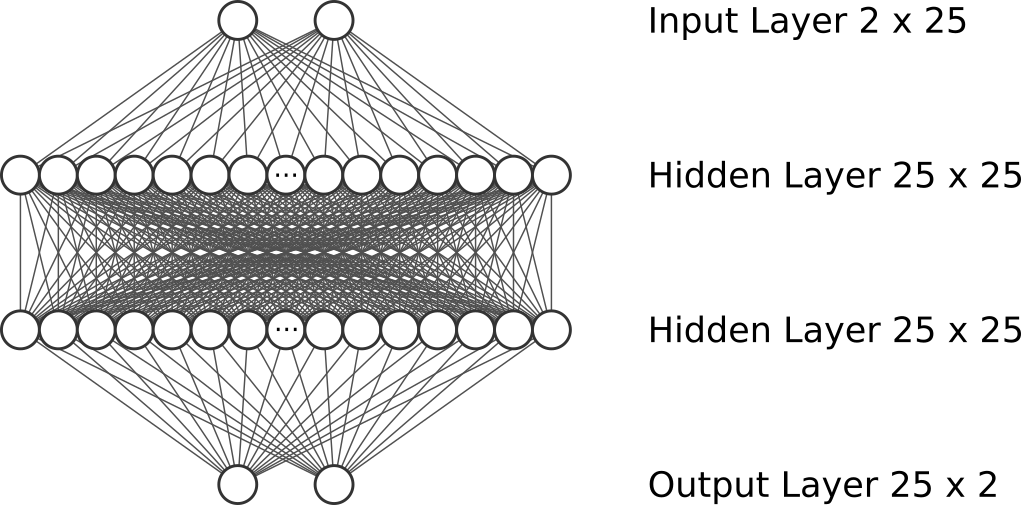
\includegraphics[width=0.45\textwidth]{figures/architecture_p2.png}
        \caption{Architecture of neural network}
        \label{fig:archi}
    \end{figure}
    

    \subsection{Datasets} % (fold)
    \label{sub:dataset}
    The train and test datasets are each composed of 1000 randomly generated samples. Each sample consists on two values chosen from a uniform distribution between 0 and 1, corresponding to a point in the 2D space. The samples that fall inside the disk of radius $1/\sqrt{2\pi}$ centered in $(0.5, 0.5)$ are labelled as 1's, whereas the rest are labelled as 0's.
    
    \subsection{Architecture} % (fold)
    \label{sub:architecture}
    
    The architecture of the system in the experiments can be found in Figure \ref{fig:archi}. It has 2 input and 2 output units and 3 fully connected layers with 25 units each. The fully connected layers are followed by a dropout layer, whose drop probability is set on the experiments. The two first hidden layers use the same activation, while the last one may use a different one. These activation functions vary depending on the experiment.


    \subsection{Results} % (fold)
    \label{sub:results}
        \begin{figure*}[t]
            \centering
            \begin{subfigure}{0.45\linewidth}
                \centering
                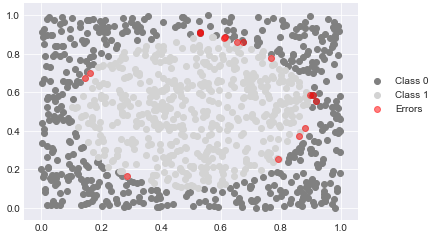
\includegraphics[width=\linewidth]{figures/res_circle_tr.png}
                \caption{Training set - 98.4\% accuracy.}
                \label{fig:rescircletr}
            \end{subfigure}%
            \begin{subfigure}{0.45\linewidth}
            \centering
            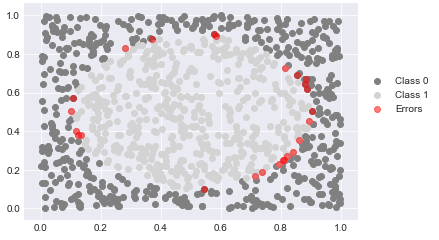
\includegraphics[width=\linewidth]{figures/res_circle_te.png}
            \caption{Test set - 97.5\% accuracy.}
            \label{fig:rescirclete}
            \end{subfigure}
            \caption{Classification results. Misclassified samples are shown in red, whereas correctly classified ones are shown in different gray levels depending on the class.}
            \label{fig:rescircle}
        \end{figure*}

        \begin{figure*}[t]
        \centering
        \begin{subfigure}{0.45\linewidth}
            \centering
            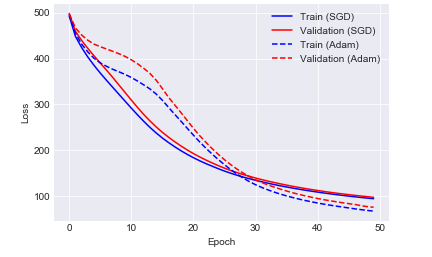
\includegraphics[width=\textwidth]{figures/adamsgdloss.png}
            \caption{Loss.}
            \label{fig:adamsgdloss}
             \end{subfigure}%
            \begin{subfigure}{0.45\linewidth}
            \centering
            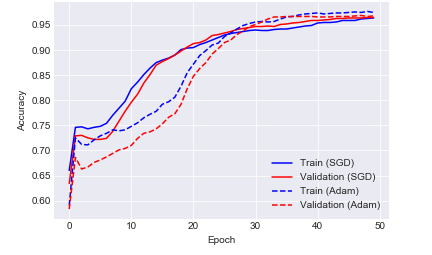
\includegraphics[width=\textwidth]{figures/adamsgdaccuracy.png}
            \caption{Accuracy.}
            \label{fig:adamsgdaccuracy}
             \end{subfigure}
             \caption{Performance per epoch using SGD and Adam.}
            \label{fig:perf_optim}
             
        \end{figure*}
        To test our framework, we evaluate the performance with three different experiments:
        
        \begin{enumerate}
            \item General performance: this experiment aims to compare the performance on the train and test sets, checking whether there is any overfitting and if dropout is needed.
            \item Comparison of the optimizers: this experiment compares the performance in terms of speed and accuracy when using \textit{Adam} or \textit{SGD} as optimizers.
            \item Comparison of the activation functions: similarly to the previous experiment, this one compares the performance with different activation functions (\textit{Tanh}, \textit{ReLU} and \textit{Leaky ReLU}) for the first two layers.
        \end{enumerate}

        All the experiments use a a batch size of 50 samples and train the model for 50 epochs.
        
        \textbf{General performance.} For the first experiment, the model uses \textit{ReLU} as the activation function for the first two fully connected layers and  \textit{Sigmoid}  for the last one. No dropout is used - i.e. it has  0 drop probability. The optimizer used is \textit{Adam} with a learning rate of $10^{-3}$, and $\beta_1 = 0.9$ and $\beta_2 = 0.999$.  The classification results obtained are shown in Figures \ref{fig:rescircletr} and \ref{fig:rescirclete}, for training and test respectively, with the misclassified samples in red. 
        

        
        The accuracy obtained for the test set is 97.5\%, very similar to the 98.4\% obtained for the training set. Hence, the model does not overfit, as could be expected since both sets are sampled from the same distribution. Therefore, we do not use dropout in any of the following experiments carried out.  It is also worth noting that all misclassified points are located in the border area.
        
        \textbf{Comparison of the optimizers.} In the second experiment we use the same architecture as in the previous one, but we train the model both with \textit{Adam} and \textit{SGD}. Adam uses the same parameters as before, while for \textit{SGD} we use the adaptive learning rate given by equation \ref{eq:lr}, with $\kappa=0.6$ and $\eta=0.035$. In Figure \ref{fig:perf_optim} can be found the loss and accuracy for the optimizers per epoch. From these figures one can observe that during the first 20 epochs, the training with SGD is faster, with a steeper slope than the one found using \textit{Adam}. However, this changes in the following epochs and  by epoch 50 both accuracy and loss are slightly better when using \textit{Adam}. Similarly to the previous experiment, there is no overfitting.
        
        

  
        \textbf{Comparison of the activation functions.}
        Lastly, we compare the results obtained using different activation functions (\textit{Tanh}, \textit{ReLU} and \textit{Leaky ReLU}) for the first two hidden layers using \textit{Adam} as optimizer. The results obtained can be observed in Figure \ref{fig:activ1comp}. In this plot we have omitted the test accuracy curves for simplicity since they were very close to their corresponding training accuracies. The accuracies obtained after 50 epochs are quite similar and do not seem to be strongly affected by the activation functions chosen for the first two activation layers. However, it is worth mentioning that \textit{Tanh} learns the fastest at first, while \textit{Leaky ReLU} seems to be the slowest.
        \begin{figure}[htp!]
            \centering
            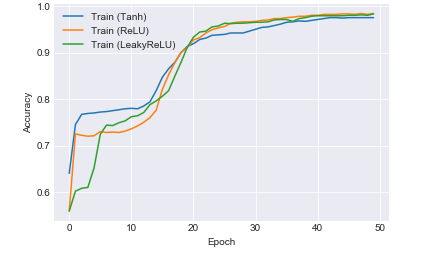
\includegraphics[width=0.45\textwidth]{figures/activ1comp.png}
            \caption{Adam's accuracy with different activation functions.}
            \label{fig:activ1comp}
        \end{figure}

\section{Conclusions} % (fold)
\label{sec:summary}
	In this project we have implemented and used a simple deep learning framework for classifying the points that fall inside and outside a disk. The performance obtained with the chosen architecture was higher than 95\% in both train and test sets after 50 epochs. Since both sets were sampled from the same distribution, there was no overfitting in the train data. The misclassified points are located in the border area, which was to be expected because a small variation in these points results in a change of their label -- whereas small changes in points that are not in the border would not modify the labels. It should also be noted that by using a well-chosen learning rate -- in this case a decaying one -- \textit{SGD} achieved a similar result to the one obtained with \textit{Adam} width default parameters.
% section summary (end)

\bibliographystyle{IEEEtran}
\bibliography{literature}

\end{document}
